\documentclass[11pt,aspectratio=169]{beamer}
\usepackage{imaxbeamer}

\title[F20 -- Endelige differanser]{Forelesning 20\\ Endelige differanser: 1D randverdiproblemer og iterasjon}
\subtitle{Kompendium §3.3 (t.o.m. Neumann-seksjonen)}
\author{IMAx3012 / IMAA3012 -- Matematikk 3B}
\date{}

\begin{document}

\begin{frame}
\titlepage
\end{frame}

\begin{frame}{I dag}
\begin{enumerate}
\item Approksimasjon av deriverte: fremover-, bakover- og sentraldifferanse.
\item 1D randverdiproblem (RVP) med Dirichlet-betingelser -- direkte løsning.
\item Iterative metoder: Jacobi- og Gauss-Seidel-iterasjon.
\item 1D RVP med Neumann-betingelser -- fiktiv rand.
\end{enumerate}
\textbf{Kode:} F20a (differanseformler), F20b (direkte/Jacobi/GS), F20c (Neumann/fiktiv rand).
\end{frame}

\section{Approksimasjon av deriverte}

\begin{frame}{Differanseformler for første og andre deriverte}
Fra definisjonen $f'(x)=\lim_{h\to0}\frac{f(x+h)-f(x)}{h}$:
\begin{defnb}{Differanseformler for første deriverte}
\[
f'(x) \approx
\begin{cases}
\dfrac{f(x+h)-f(x)}{h}, & \text{fremoverdifferanse} \\
\dfrac{f(x)-f(x-h)}{h}, & \text{bakoverdifferanse} \\
\dfrac{f(x+h)-f(x-h)}{2h}, & \text{sentraldifferanse (snitt av de to over)}
\end{cases}
\]
\end{defnb}
\begin{defnb}{Differanseformel for andre deriverte}
\[
f''(x) \approx \frac{f(x+h)-2f(x)+f(x-h)}{h^2}.
\]
\end{defnb}
\end{frame}

\begin{frame}{Geometrisk tolkning: sekantlinjer}
Hver formel er stigningstallet til en sekantlinje gjennom punkter på grafen til $f$. Sentraldifferansens sekant (gjennom $x_0\pm h$) ligger tettest opptil tangenten.
\begin{center}
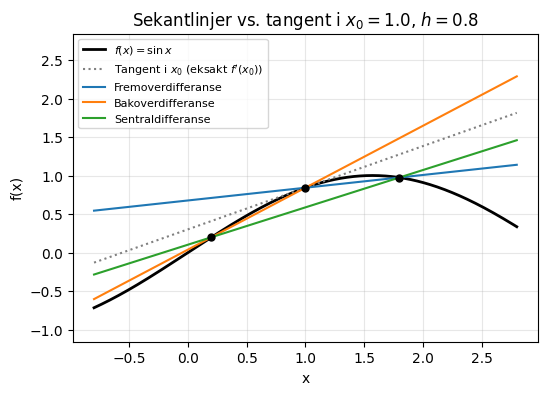
\includegraphics[width=0.72\textwidth]{assets/secant_tangent.png}
\end{center}
\end{frame}

\begin{frame}{Konvergensorden: $O(h)$ vs. $O(h^2)$}
\begin{columns}
\begin{column}{0.5\textwidth}
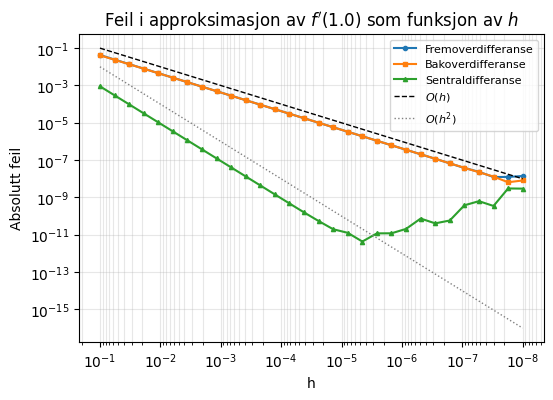
\includegraphics[width=\textwidth]{assets/order_h_h2.png}
\end{column}
\begin{column}{0.5\textwidth}
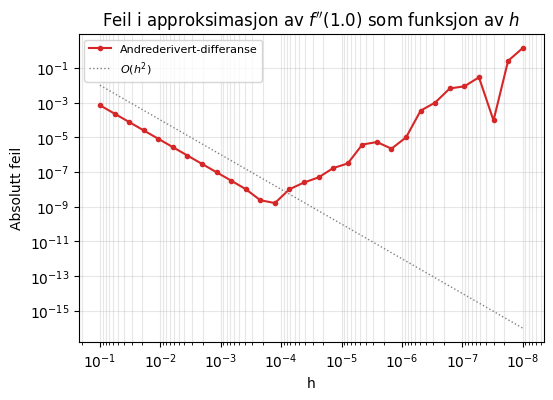
\includegraphics[width=\textwidth]{assets/order_second_deriv.png}
\end{column}
\end{columns}
Fremover/bakover: $O(h)$ (feilen halveres når $h$ halveres). Sentraldifferanse og 2.derivert-formelen: $O(h^2)$ (feilen firedobles når $h$ dobles) -- systematisk mer nøyaktig.
\end{frame}

\section{1D Randverdiproblem med Dirichlet-betingelser}

\begin{frame}{Problemstilling}
\[
u'' + p(x)u' + q(x)u = r(x), \quad a\le x\le b, \quad u(a)=u_a,\ u(b)=u_b.
\]
\textbf{Metode} (grovt sett, generelt for endelige differanser):
\begin{enumerate}
\item Diskretiser definisjonsmengden.
\item Erstatt deriverte med approksimasjoner i hvert rutenettpunkt.
\item Erstatt eksakt løsning med dens approksimasjon $U_i$.
\item Løs det resulterende ligningssystemet.
\end{enumerate}
Velg $N$, $h=(b-a)/N$, $x_i=a+ih$, $i=0,\ldots,N$ (indre punkter: $i=1,\ldots,N-1$).
\end{frame}

\begin{frame}{Diskretisering: den tridiagonale strukturen}
Sentraldifferanser i hvert indre punkt, multiplisert med $h^2$, gir -- etter å samle ledd i $U_{i-1},U_i,U_{i+1}$:
\begin{equation}
v_i U_{i-1} + d_i U_i + w_i U_{i+1} = h^2 r(x_i), \quad i=1,\ldots,N-1,
\end{equation}
der
\[
v_i = 1-\tfrac{h}{2}p(x_i), \qquad d_i = -2+h^2q(x_i), \qquad w_i = 1+\tfrac{h}{2}p(x_i).
\]
Hver ligning involverer kun $U_{i-1},U_i,U_{i+1}$ -- dette gir den tridiagonale matrisen $A$:
\[
A = \begin{bmatrix}
1 & & & & \\
v_1 & d_1 & w_1 & & \\
 & \ddots & \ddots & \ddots & \\
 & & v_{N-1} & d_{N-1} & w_{N-1} \\
 & & & 0 & 1
\end{bmatrix}, \qquad \vect b = \big[u_a,\, h^2r(x_1),\,\ldots,\,h^2r(x_{N-1}),\, u_b\big]^T.
\]
Løs $A\vect U=\vect b$.
\end{frame}

\begin{frame}{Eksempel: Dirichlet-RVP}
\[
u''+2u'-3u=9x, \quad u(0)=u_a=1, \quad u(1)=u_b=e^{-3}+2e^{-5}=0.486351,
\]
eksakt løsning $u(x)=e^{-3x}+2e^x-3x-2$. Med $N=4$, $h=0.25$:
\[
\begin{bmatrix}
1 & & & & \\
0.75 & -2.1875 & 1.25 & & \\
 & 0.75 & -2.1875 & 1.25 & \\
 & & 0.75 & -2.1875 & 1.25 \\
 & & & & 1
\end{bmatrix}\!
\begin{bmatrix}U_0\\U_1\\U_2\\U_3\\U_4\end{bmatrix}
=
\begin{bmatrix}1\\0.140625\\0.28125\\0.421875\\0.486351\end{bmatrix}
\]
Løsning: $U_1=0.293176,\ U_2=0.025557,\ U_3=0.093820$ -- svært nær eksakte verdier $u(0.25)=0.290417$, $u(0.5)=0.020573$, $u(0.75)=0.089400$.
\end{frame}

\begin{frame}[fragile]{Implementering (F20b)}
\begin{lstb}[los\_RVP\_direkte -- konstante p,q]
\begin{verbatim}
def los_RVP_direkte(p, q, r_func, a, b, ua, ub, N):
    h = (b - a) / N
    x = a + h * np.arange(N + 1)
    v, d, w = 1 - h/2*p, -2 + h**2*q, 1 + h/2*p
    A = ...tridiag(v, d, w)...         # NxN, med rand-rader = 1
    bvec = h**2 * r_func(x)
    bvec[0], bvec[-1] = ua, ub
    U = np.linalg.solve(A, bvec)
    return x, U
\end{verbatim}
\end{lstb}
\begin{center}
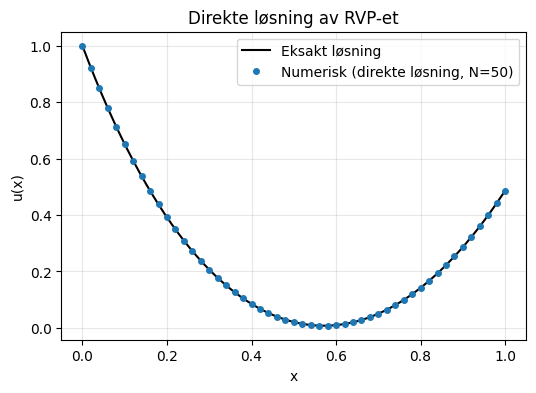
\includegraphics[width=0.6\textwidth]{assets/direkte_vs_eksakt.png}
\end{center}
\end{frame}

\section{Jacobi- og Gauss-Seidel-iterasjon}

\begin{frame}{Hvorfor iterative metoder?}
Å løse $A\vect U=\vect b$ direkte fungerer fint i 1D. Men i 2D (neste forelesning) blir $A$ stor og upraktisk å sette opp eksplisitt.
\begin{remb}{Iterative metoder}
Start med en gjetning, forbedre den gradvis -- uten noen gang å sette opp eller faktorisere $A$. Løs ligningen $v_iU_{i-1}+d_iU_i+w_iU_{i+1}=h^2r(x_i)$ for $U_i$:
\[
U_i = \frac{1}{d_i}\Big(h^2r(x_i) - v_iU_{i-1} - w_iU_{i+1}\Big).
\]
\end{remb}
Bruk dette som oppdateringsformel: de to metodene skiller seg kun i hvilke naboverdier som brukes.
\end{frame}

\begin{frame}{Jacobi vs. Gauss-Seidel}
\begin{defnb}{Jacobi-iterasjon}
\[
U_i^{(m+1)} = \frac{1}{d_i}\Big(h^2r(x_i) - v_iU_{i-1}^{(m)} - w_iU_{i+1}^{(m)}\Big).
\]
Alle verdier hentet fra \emph{forrige} iterasjon $U^{(m)}$.
\end{defnb}
\begin{defnb}{Gauss-Seidel-iterasjon}
\[
U_i^{(m+1)} = \frac{1}{d_i}\Big(h^2r(x_i) - v_iU_{i-1}^{(m+1)} - w_iU_{i+1}^{(m)}\Big).
\]
Bruker \emph{oppdaterte} verdier så snart de er tilgjengelige.
\end{defnb}
Begge itereres til $\max_i|U_i^{(m+1)}-U_i^{(m)}|<$ toleranse.
\end{frame}

\begin{frame}{Eksempel: konvergenshastighet}
$u''=0$ på $[0,2]$, $u(0)=20$, $u(2)=50$ (eksakt: $u(x)=20+15x$). Med $N=10$, toleranse $10^{-8}$:
\begin{center}
\begin{tabular}{lcc}
\toprule
 & Jacobi & Gauss-Seidel \\
\midrule
Antall iterasjoner & 398 & 201 \\
\bottomrule
\end{tabular}
\end{center}
\begin{center}
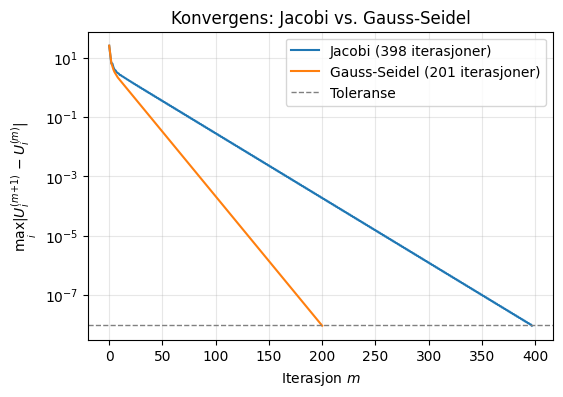
\includegraphics[width=0.62\textwidth]{assets/jacobi_gs_konvergens.png}
\end{center}
Gauss-Seidel bruker info så snart den er tilgjengelig -- konvergerer typisk om lag dobbelt så raskt, for omtrent samme arbeid per iterasjon. Generaliserer direkte til 2D (F21) -- der blir det faktisk den foretrukne metoden.
\end{frame}

\begin{frame}{Virker like fint for $r(x)\neq0$}
Samme kode, uendret -- Poisson-type eksempel $u''=-\cos(3x)$:
\begin{center}
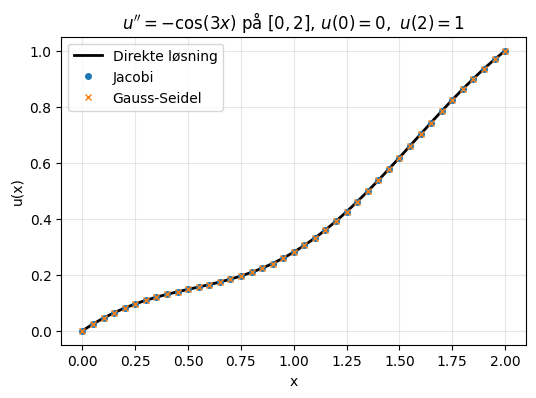
\includegraphics[width=0.62\textwidth]{assets/poisson_type_eksempel.png}
\end{center}
\end{frame}

\section{1D Randverdiproblem med Neumann-betingelser}

\begin{frame}{Problemet: $U_0$ er nå ukjent}
\[
u'' + p(x)u' + q(x)u = r(x), \quad u'(a)=u_a', \quad u(b)=u_b.
\]
I Dirichlet-tilfellet var $U_0=u_a$ gitt direkte -- triviell ligning. Nå er $u(a)$ ukjent: $U_0$ er en ekte ukjent, og vi trenger en ny ligning i $x_0=a$.
\begin{remb}{Hvorfor ikke bare en enkel fremoverdifferanse?}
$u_a' \approx \frac{U_1-U_0}{h}$ er bare \emph{førsteordens} -- lavere nøyaktighet enn resten av skjemaet (som er $O(h^2)$). En andreordens formel med $x_0,x_1,x_2$ ødelegger den tridiagonale strukturen. Løsning: \emph{fiktiv rand}.
\end{remb}
\end{frame}

\begin{frame}{Ideen: en fiktiv rand}
Tenk at løsningen er definert i et fiktivt punkt $x_{-1}=a-h$, med ukjent $U_{-1}$:
\begin{center}
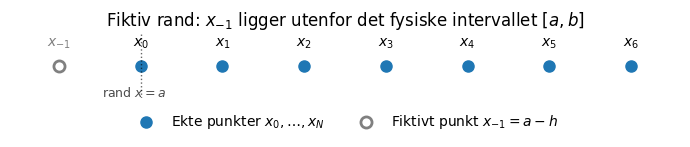
\includegraphics[width=0.75\textwidth]{assets/fiktiv_rand_gitter.png}
\end{center}
\[
\frac{U_1-2U_0+U_{-1}}{h^2} + p(x_0)\frac{U_1-U_{-1}}{2h} + q(x_0)U_0 = r(x_0), \qquad
\frac{U_1-U_{-1}}{2h} = u_a'.
\]
Løs den andre for $U_{-1}=U_1-2hu_a'$ og sett inn i den første -- eliminerer den fiktive ukjente, og beholder sentraldifferanser (dermed $O(h^2)$) begge steder.
\end{frame}

\begin{frame}{Modifisert ligning ved $x_0$}
\[
\frac{2U_1-2U_0-2hu_a'}{h^2} + p(x_0)u_a' + q(x_0)U_0 = r(x_0).
\]
Kun \emph{denne} ligningen endres -- resten av det tridiagonale systemet er uendret.
\begin{eksb}{Neumann-betingelse}
\footnotesize Samme ligning som Dirichlet-eksempelet, men $u'(0)=u_a'=-4$ i stedet for $u(0)=1$ (samme eksakte løsning). Med $N=4,h=0.25$: $U_0=0.92103219,\ U_1=0.25737896,\ U_2=0.01029386,\ U_3=0.08858688.$
\end{eksb}
\begin{center}
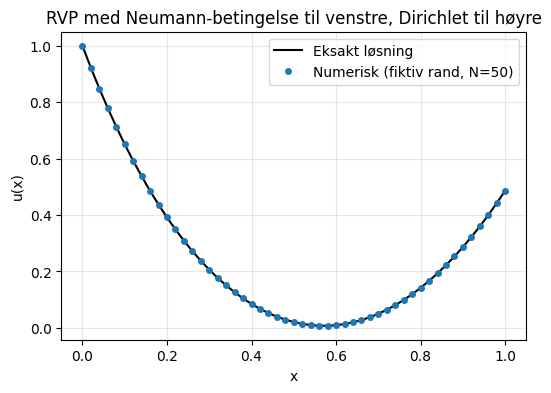
\includegraphics[width=0.33\textwidth]{assets/neumann_vs_eksakt.png}
\end{center}
\end{frame}

\begin{frame}{Lønner den fiktive randen seg?}
Sammenlign konvergensorden: fiktiv rand (sentraldifferanse begge steder) vs. naiv fremoverdifferanse for $u_a'$.
\begin{columns}
\begin{column}{0.55\textwidth}
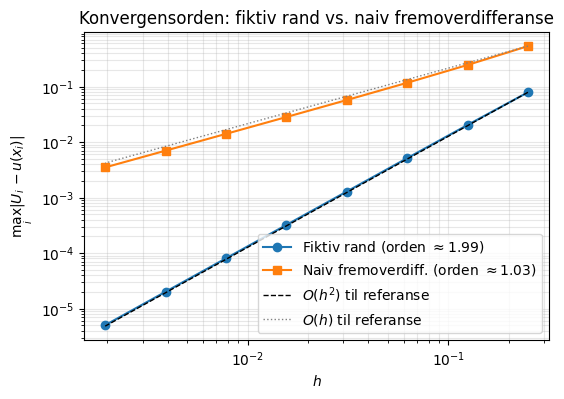
\includegraphics[width=\textwidth]{assets/neumann_konvergensorden.png}
\end{column}
\begin{column}{0.45\textwidth}
\begin{remb}{Målt orden (F20c)}
\footnotesize Fiktiv rand: $\approx 1.99$ ($O(h^2)$, som Dirichlet). Naiv fremoverdiff.: $\approx 1.03$ ($O(h)$) -- selv om kun \emph{ett} endepunkt behandles annerledes, ødelegger det nøyaktigheten i hele løsningen.
\end{remb}
\end{column}
\end{columns}
\end{frame}

\begin{frame}{Oppsummering}
\begin{itemize}
\item Sentraldifferanse er $O(h^2)$ og foretrekkes over de ensidige formlene ($O(h)$), bortsett fra ved endepunkter.
\item Dirichlet-RVP $\Rightarrow$ tridiagonalt system $A\vect U=\vect b$, løst direkte eller med Jacobi/Gauss-Seidel.
\item Gauss-Seidel konvergerer typisk $\sim2\times$ raskere enn Jacobi.
\item Neumann-betingelser krever en ekstra ligning ved randen -- fiktiv rand bevarer $O(h^2)$-nøyaktigheten i hele løsningen.
\end{itemize}
\end{frame}

\begin{frame}{Neste gang: F21 -- 2D og varmeligningen}
\begin{nestefb}
Samme ideer (fempunktsformel, Jacobi/Gauss-Seidel) generaliseres til \emph{to} romdimensjoner for Laplace-/Poisson-ligningen. Deretter: det første eksempelet på en \emph{tidsavhengig} PDE -- varmeligningen, løst med semi-diskretisering og eksplisitt Euler.
\end{nestefb}
\end{frame}

\end{document}
